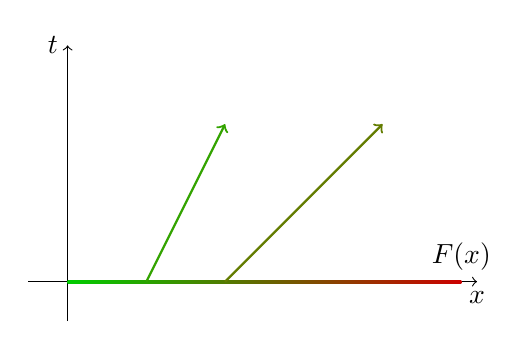
\begin{tikzpicture}


\draw[->] (-0.5, 0) -- (5.2,0) node[below] {$x$};
\draw[->] (0, -0.5) -- (0,3) node[left] {$t$};

\fill[left color = green!80!black, right color = red!80!black] (0,-0.02) rectangle (5, 0.02) node[above] {$F(x)$};

\draw[thick, green!80!black!80!red, ->] (1,0) -- (2,2);
\draw[green!80!black!61!red, thick, ->] (2,0) -- (4,2);

\end{tikzpicture}
